\documentclass[a4paper, 10pt]{article}
\usepackage[utf8]{inputenc} % Change according your file encoding
\usepackage{graphicx}
\usepackage{url}

%opening
\title{Seminar Report: Namy}
\date{\normalsize\today{}}

\begin{document}
\author{}
\maketitle

\begin{center}
  \textbf{Carles Tornel}\\
  \textbf{Jesus Alfaro}\\
  \textbf{Ricard Abril}

\end{center}
\section{Introduction}
En aquesta pràctica haurem d'implementar un
servidor de noms distribuïts on s'emmagatzemaran
els identificadors dels processos hosts. S'utilitzarà el sistema de cache, però, com el TTL per defecte és 0, no hi haurà intervenció de la cache a la primera versió, a la segona versió demana modificar aquest valor per tal de fer servir la cache.

\newpage\section{Experiments}

\subsection{Testing}
\subsubsection{Make experiments with several clients asking for name resolution concurrently}
En aquest primer experiment hem iniciat els diferents nodes tot seguint les indicacions de la documentació, després hem iniciat la resolució de www, upc i edu en diversos clients de forma concurrent tal com podem veure a la imatge següent:\\\\
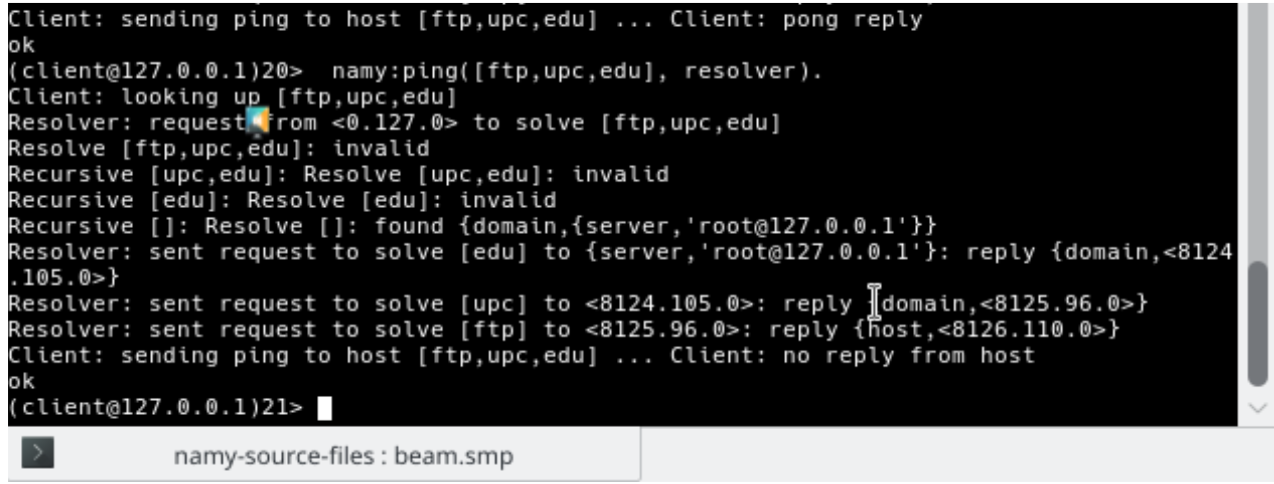
\includegraphics[width=\textwidth]{Ex1.png}\\\\
\subsubsection{Shut down a host (by sending a stop message) and try to solve its name again.}
Simplement, la petició no podrà ser atesa, de forma que saltara el timeout i obtindrem un missatge d'error.
\newpage\subsubsection{Modify the server and the host code so that when they are shut down, they unregister their entry in their corresponding parent domain and repeat the last experiment}
Amb aquesta modificació, quan eliminem un host, aquest és eliminat en el seu pare, de forma que quan intentem resoldre'l, en canvi d'obtenir un error a causa del timeout rebem la resposta del pare dient que no pot trobar el host en qüestió, tal com podem veure en la següent imatge:\\\\
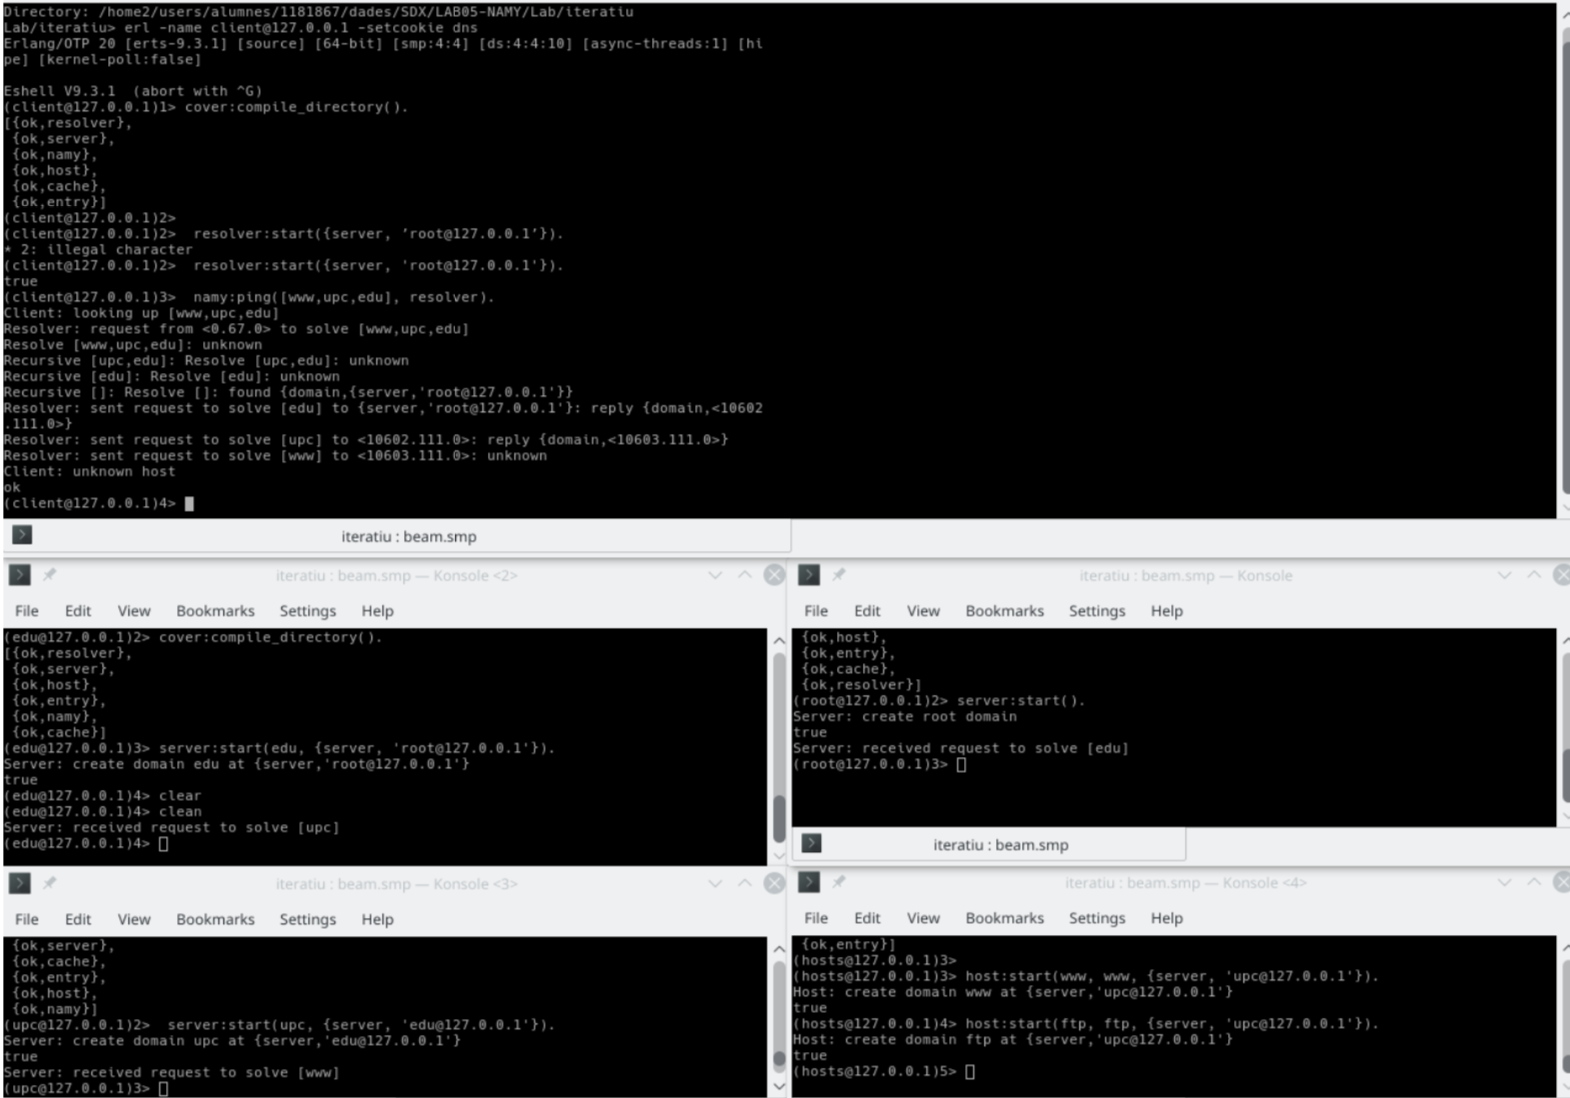
\includegraphics[width=\textwidth]{Ex2.png}\\\\
\subsection{Using the cache}
\subsubsection{Set a long TTL (i.e. minutes) and ’move’ a host (i.e. query for a host name, shut it down, start it up registered under the same name, and finally query it again).}
Si assignem un TTL més alt, les resolucions tardaran més a ser esborrades de la cache, de forma que si movem el host i intentem fer una petició ha aquest abans d'haver resolt de nou, no obtindrem cap resposta, ja que aquell host ja no es troba en l'adreça a la qual estem fent ping.
\newpage\subsubsection{Derive a theoretical quantification of the amount of messages needed for name resolution without and with the cache and check experimentally that your formulation is correct (assume a resolver that repeats the same query about a host at depth D in the namespace every F seconds for a total duration of R seconds, being the TTL equal to T seconds).}
Per realitzar aquest experiment em assignat un TTL de 600 (en el cas que utilitzem la cache) i un TTL de 0 en el cas que no volem utilitzar la cache.\\
El número de pings obtinguts amb cache és de 32305, en canvi quan no utilitzem la cache el número de pings és de 15437.\\
Sense utilitzar la cache podem veure que obtenim menys pings, però generarà un tràfic molt major a la xarxa, en el cas que utilitzem cache, només ens caldran 32310 missatges, per a fer 32304 pings, però en el cas de no utilitzar la cache ens caldran 123496 missatges per poder fer 15437 pings. En la imatge següent observem les diferències en l'execució d'ambdós "models".\\\\
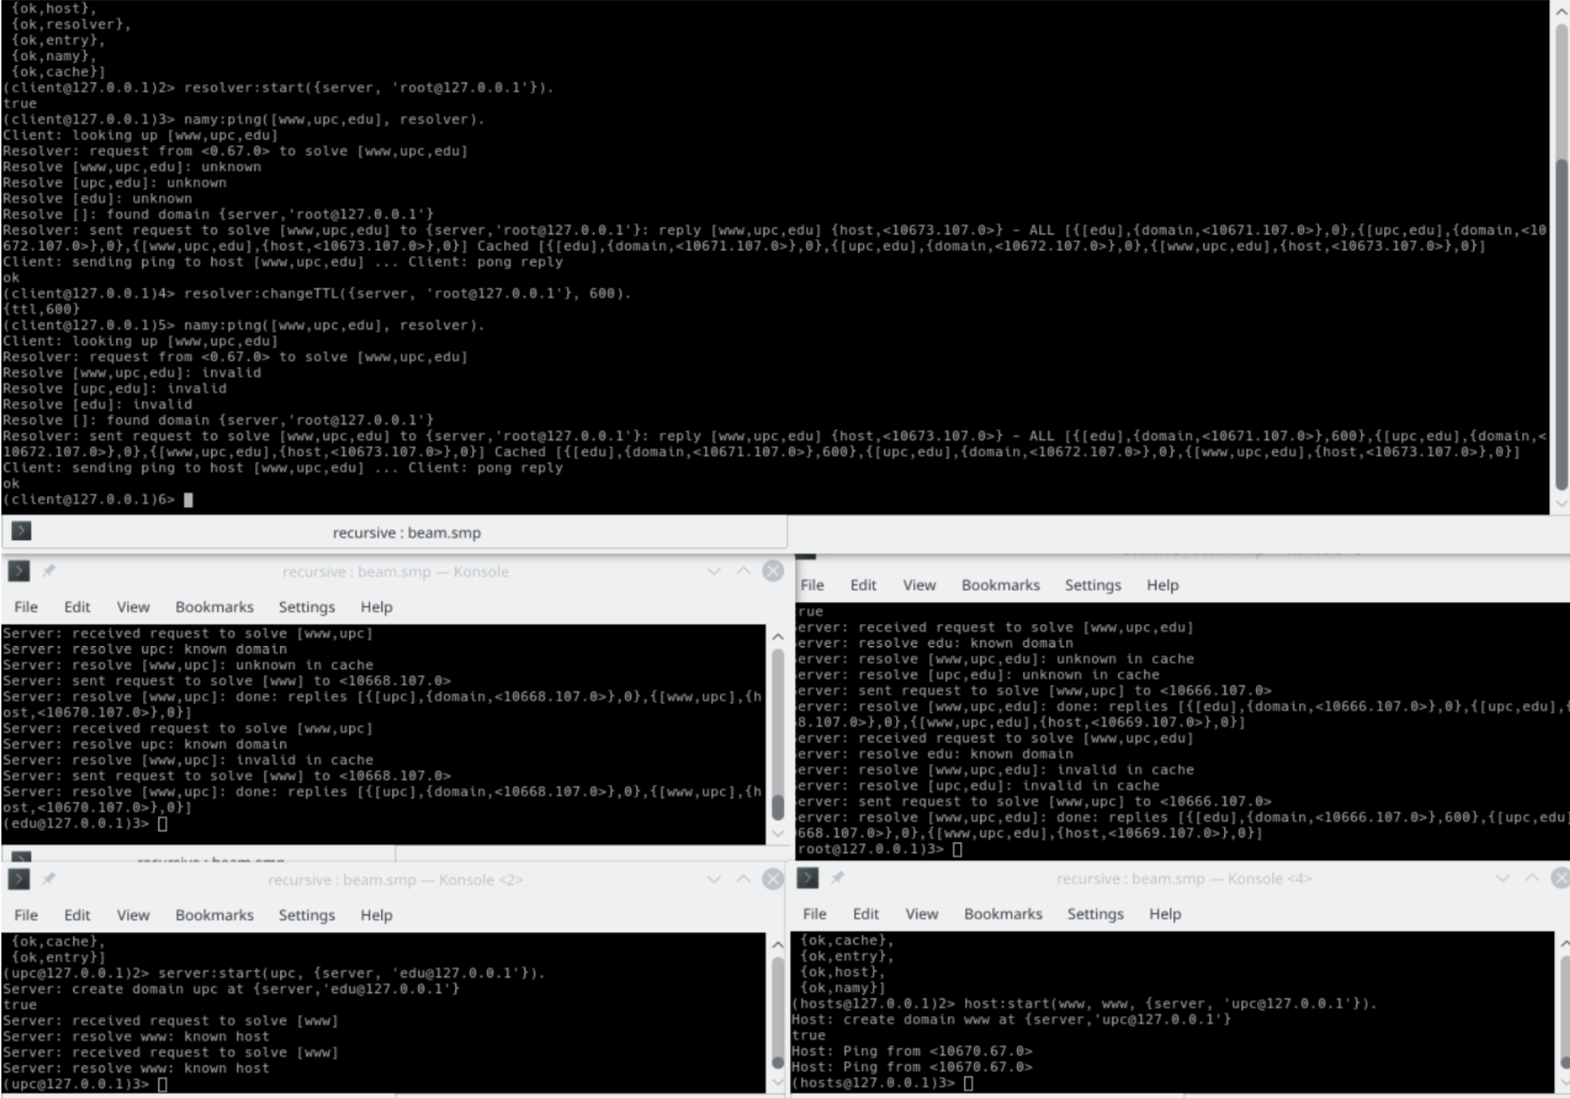
\includegraphics[width=\textwidth]{Ex3.png}

\newpage
\subsection{Recursive resolution}
\subsubsection{Set up the naming system by using the new versions of the resolver and the server that implement recursive resolution. Perform exper- iments to compare this version with the former one using iterative resolution. Focus especially on how caching performs on each one when using several clients.}
En aquest experiment, hem assignat un TTL de 0 per la implementació recursiva i per l'implementació iterativa, després hem fet el mateix amb un TTL de 3.\\
Per provar els diferents models, hem posat el sistema en funcionament durant mig minut aproximadament.\\
Pel model recursiu amb TTL 0, hem obtingut 8862 pings.\\
Pel model iteratiu amb TTL 0, hem obtingut 12891 pings.\\
 En canvi per el model amb TTL 3, hem obtingut:\\
Pel model recursiu 49589.\\ 
Pel model iteratiu 50120.\\ 
Per tant podem concloure que la versió iterativa serà més rapida. Tal com podem veure en la imatge següent:\\\\
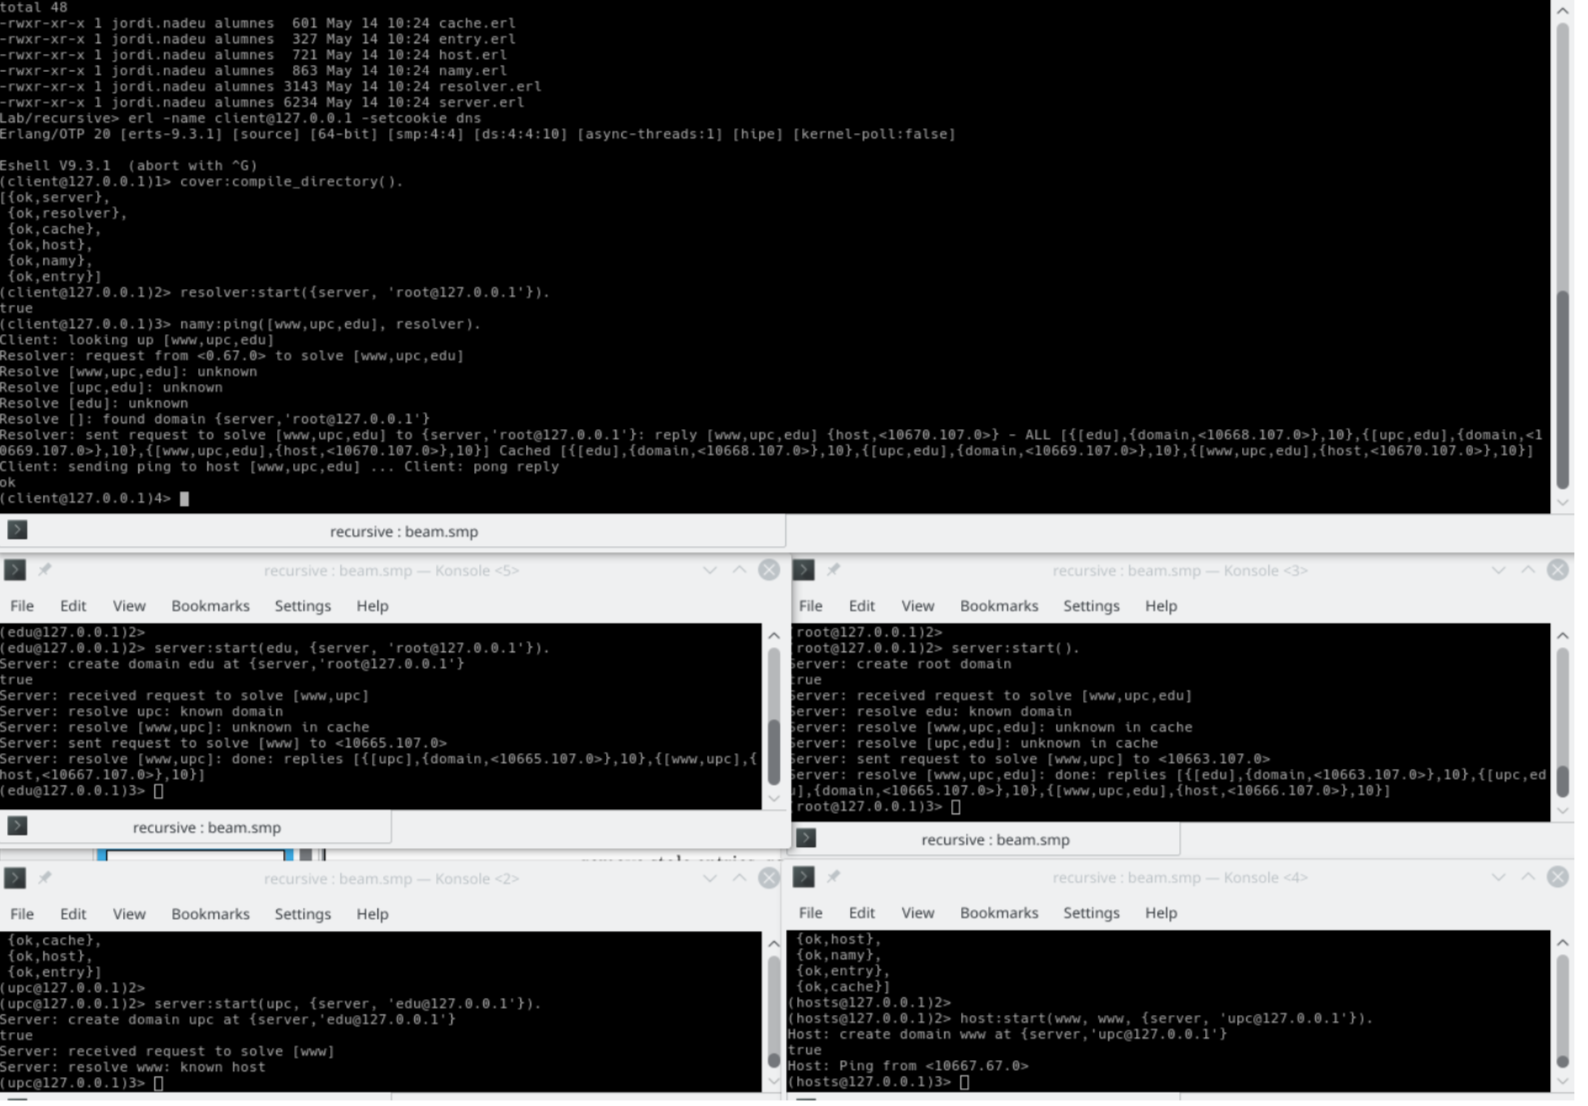
\includegraphics[width=\textwidth]{Ex5.png}

\newpage\section{Open Questions}
\section{Testing}
\subsubsection{ What is the observed behavior?}
El comportament després de tancar el host i tornar a resoldre el seu nom, serà el mateix que quan es fa per primera vegada la resolució, ja que les entrades de cache tenen TTL 0, i per tant no estarà disponible per al client.
\subsubsection{ What is different now?}
Using the cache
\subsubsection{ What is the observed behavior?}
Una vegada el resolver rep una resposta dels servidors, la guarda a una entrada de cache amb el TTL corresponent, en segons, i quan torni a rebre una petició d'un client, en l'interval indicat pels segons, podrà saltar-se la resolució i retornar el resultat de l'entrada de cache corresponent.
\subsubsection{ What happened with cached information in the resolver? Which nodes need to be notified about the host movement?}
La informació de cache estaràn disponible per als clients segons el temps TTL ho indiqui. Com el resolver fa les peticions iterativament, la càrrega de treball es major, i per tant, tardarà més temps en satisfer les peticions dels clients. A més, si el TTL és petit pot resultar poc eficient perquè el resolver haurà de tornar a fer tot el treball una vegada més, i pot no haver gaire diferencia amb una cache de 0 TTL.\\
Els nodes que hauran de ser notificats per un moviment de hosts son 
els que pertanyen al administrational i managerial layer, i que estiguin a un nivell superior al host desplaçat, els pares del host.
\subsection{Recursive Resolution}
\subsubsection{ Which version can exploit caching better? Justify why.}
L'escenari on ens trobem determinarà si una solució és millor que una altra.
\\El temps de càlcul d'inserció i d'extracció es capaç de ralentitzar una petició qualsevol, fins i tot quan les llistes no han presentat més de 3 elements, segons s'ha pogut observar a la realització dels experiments.\\
És més favorable utilitzar la sol·lució recursiva en un escenari on el Time To Live és considerablement gran i hi han moltes peticions de clients per un mateix host, però en el nostre cas (amb un TTL menor i molts hosts) és millor utilitzar la sol·lució iterativa.

\newpage\section{Personal opinion}
    Aquest laboratori ha ajudat a clarificar un dels conceptes més comuns dels sistemes distribuïts en xarxa: La communicació multicast. Mitjançant la pràctica de l'implementació de nodes com poden ser els Workers, Leaders i Slaves, es té una visió més exemplificadora del problema que s'ha tractat.
\end{document}
